% vim: spell spelllang=en_gb
\chapter{Results}

This section presents the results of the methods used in the project, including the text classifier,
and the evaluation of the pipeline by applying it to unlabelled data and checking the visual
interface.


\section{Text Classification}
Table~\ref{tab:metrics} shows the evaluation metrics for the trained DistilBERT model on the dataset
and a balanced version by doing undersampling. Table~\ref{tab:tweets_missclassified} shows falsely
classified tweets from the Swedish dataset translated to English.

\begin{table}
      \center
      \bgroup
      \def\arraystretch{1.5}
  \begin{tabular}{|c|c|c|c|c|c|}
    \hline
            & Accuracy & Precision & Recall & F$_1$ Score & Confusion Matrix\\
    \hline
    Original & 0.9231 & 0.8944 & 0.9181 & 0.9061 &
    $
    \begin{bmatrix}
      381 & 34 \\ 
      568 & 45
\end{bmatrix}
$\\
    \hline
    Undersampled & 0.9137 & 0.9091 & 0.9138 & 0.9115 &
    $
    \begin{bmatrix}
      350 & 33\\ 
      370 & 35
    \end{bmatrix}
    $\\
    \hline
  \end{tabular}
      \egroup
      \caption{Evaluation metrics}
      \label{tab:metrics}
\end{table}

\begin{table}
      \center
      \begin{tabular}{|p{5cm}|p{5cm}|l|l|}
    \hline
    Translated tweet & Processed tweet & Predicted label & Actual label\\
    \hline
    The road has rained away outside our driveway!! Damn storm https://t.co/wU6uuZo7El &
    road rained away outside driveway damn storm & 0 & 1 \\
    \hline
 Right now! Stormy weather in southern Norway. Functionality affected - all resources prioritized to save lives, correct in Vestfold. &
 right stormy weather southern norway functionality affected resources prioritized save lives correct vestfold & 0 & 1\\
    \hline
 AFTER LIGHT! Basement full of water? Do you live in \#Stockholm and are affected by this weekend's
 \#flooding? Call reporter Nadya bums &
 light basement water live affected weekends reporter nadya bums & 0 & 1\\
    \hline
 Impressed by efforts and people's patience. Here is the latest municipal information. \#Hallsberg
 \#Flooding \#orepol \#svpol http://t.co/C0sCxEDtLT &
 impressed efforts peoples patience latest municipal information & 0 & 1 \\
    \hline
     world Floods, war, famine, terror. Goodnight world. & 
 floods war famine terror goodnight & 1 & 0 \\
    \hline
     Flooding in the bathtub? & 
 flooding bathtub & 1 & 0 \\
    \hline
 A basement was flooded when a water main leaked in \#Vårberga in \#Borgå \#borgåvatten https://t.co/zX08QDqJv9 & 
 basement flooded water main leaked & 1 & 0 \\
    \hline
 storm flood assumption years Storm flood assumption off by about 2,500 years https://t.co/v14XtEcbTC & 
 storm flood assumption years & 1 & 0 \\
    \hline
  \end{tabular}
      \caption{Miss-classified tweets}
      \label{tab:tweets_missclassified}
  \end{table}


\section{Visualization}
 Visualization is often placed at the end of the pipeline and might be the most important since it
brings meaning to the results, which can be interrupted by most audiences. Also, it's a direct way
to verify that the pipeline is working. The web application is made by
Dash\footnote{https://dash.plotly.com/} to create an interface for
Plotly\footnote{https://plotly.com/python/}'s visualizations. Dash Bootstrap
Components\footnote{https://dash-bootstrap-components.opensource.faculty.ai/} is used as well for
an easier way to use Bootstrap components for Plotly Dash, such as buttons, input, and tables.


Figure~\ref{fig:visual_interface} shows the visual interface containing all the graphs enabling spatial, temporal, and
textual exploration of the tweets. Users can add filtering rules for the tweets in all the plots
using their creation dates, location, and textual properties.

\begin{figure}[H]
\begin{center}
  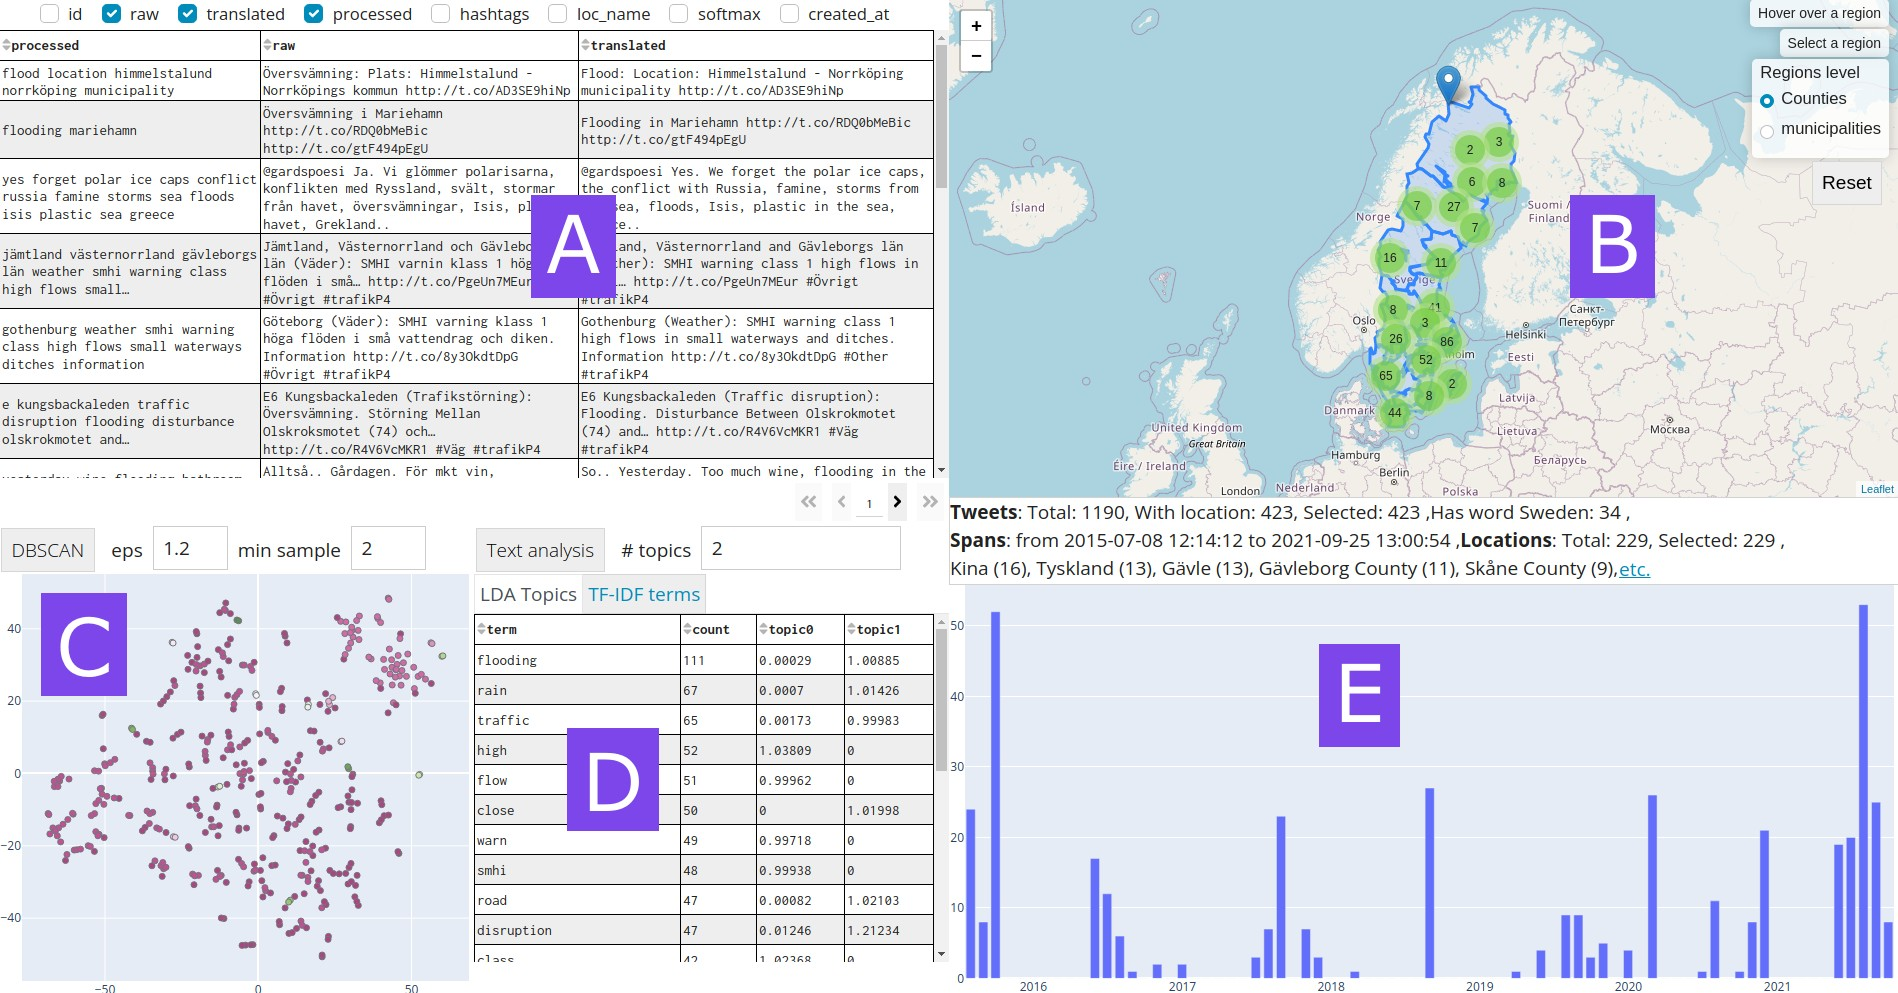
\includegraphics[width=\columnwidth]{./images/visual_interface.png}
\end{center}
\caption{Visual interface}
\label{fig:visual_interface}
\end{figure}


Figure~\ref{fig:map} shows an interactive map containing clickable clustered pointers for the
tweets. The clusters disperse or congregate upon zooming in or zooming out, respectively. Hovering
over a pointer shows the pop-up with the location name extracted by the pipeline. Clicking on a
cluster of a region select the tweets they contain; this will zoom in to cover them while filtering
out the unselected pointers from the map. The top left section of the map has several elements: text
elements to show the name of the hovered and selected regions, a radio element to change the level
of regions that can be selected between counties and municipalities, and a reset button to remove
the filter by showing all the pointers.

\begin{figure}[H]
\begin{center}
  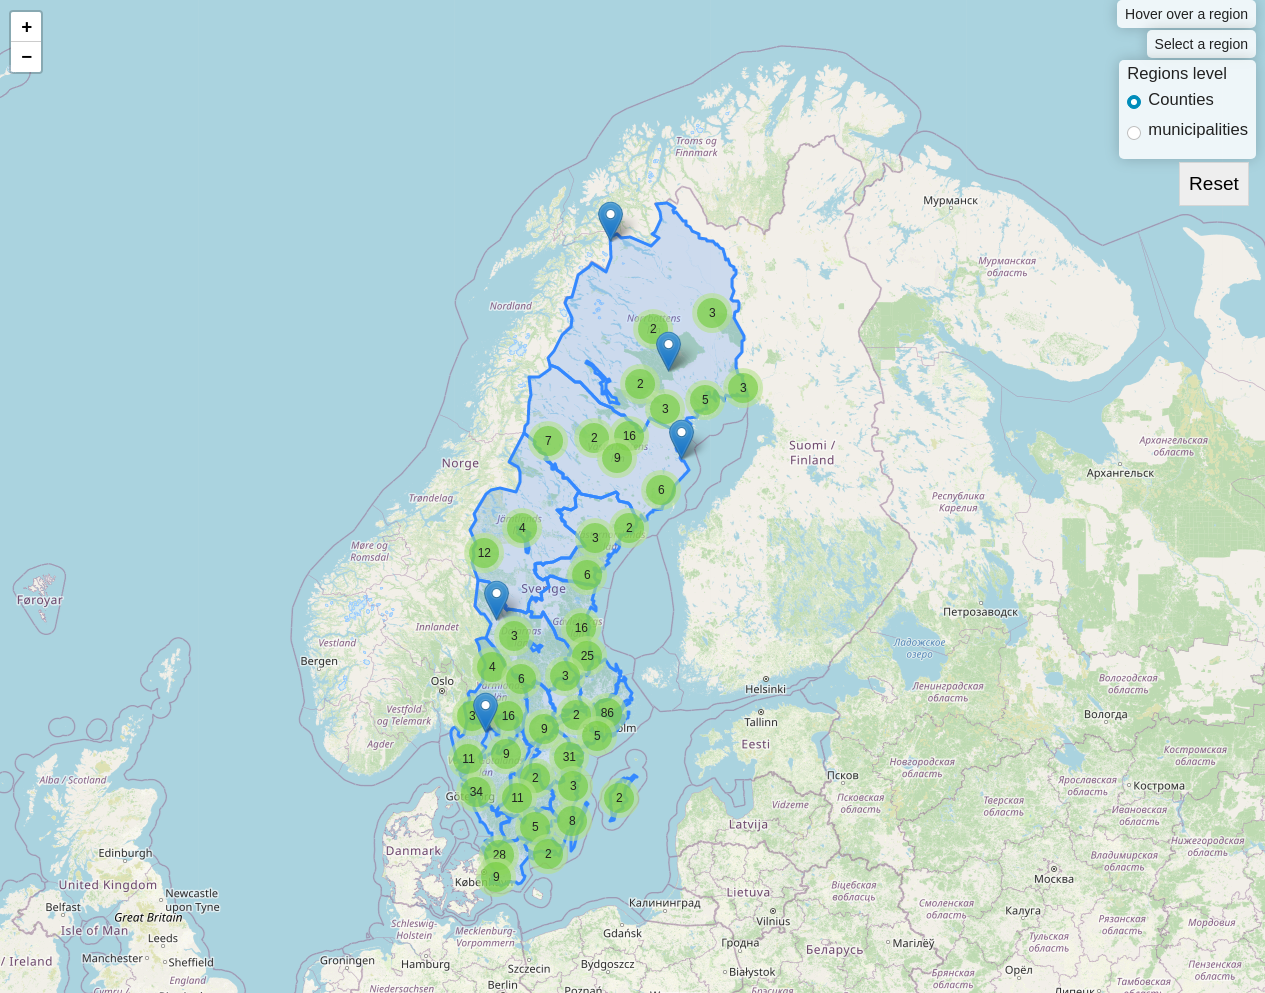
\includegraphics[width=\columnwidth]{./images/map.png}
\end{center}
\caption{Map showing clusters of tweets}
\label{fig:map}
\end{figure}


Another way to explore the tweets is by using the histogram for their creation date as seen in
Figure~\ref{fig:histogram}. The dates are aggregated by day if they span a month or less; otherwise, by month.
Selecting the tweets can be done by using a select box between two dates. Hovering over the bars
show the date and the number of tweets, and the blue and red parts of the bars represents the selected
and unselected tweets, respectively.

\begin{figure}[H]
\begin{center}
  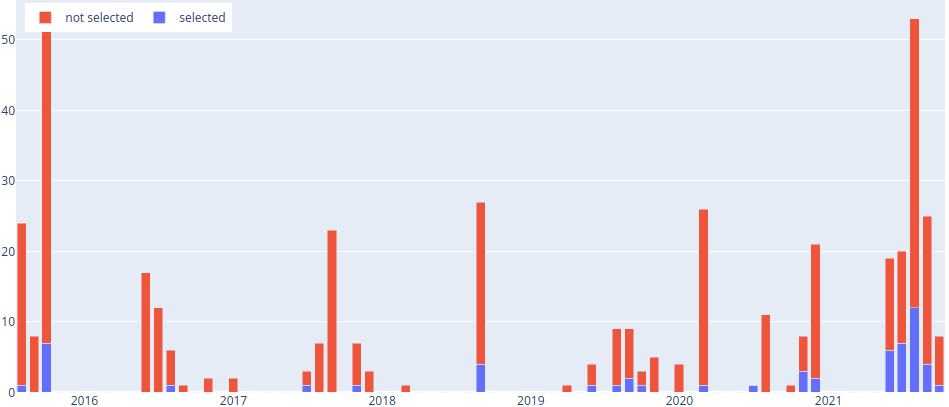
\includegraphics[width=\columnwidth]{./images/histogram.png}
\end{center}
\caption{Histogram for tweets' creation dates}
\label{fig:histogram}
\end{figure}

The table in Figure~\ref{fig:tweets_table} shows the selected tweets with several of its attributes: the ID, the raw
(original) text, the translated text, the processed text, the hashtags used, the location extracted,
the softmax value for the prediction, and the creation date. It's sortable by column and the rows
are paginated.

\begin{figure}[H]
\begin{center}
  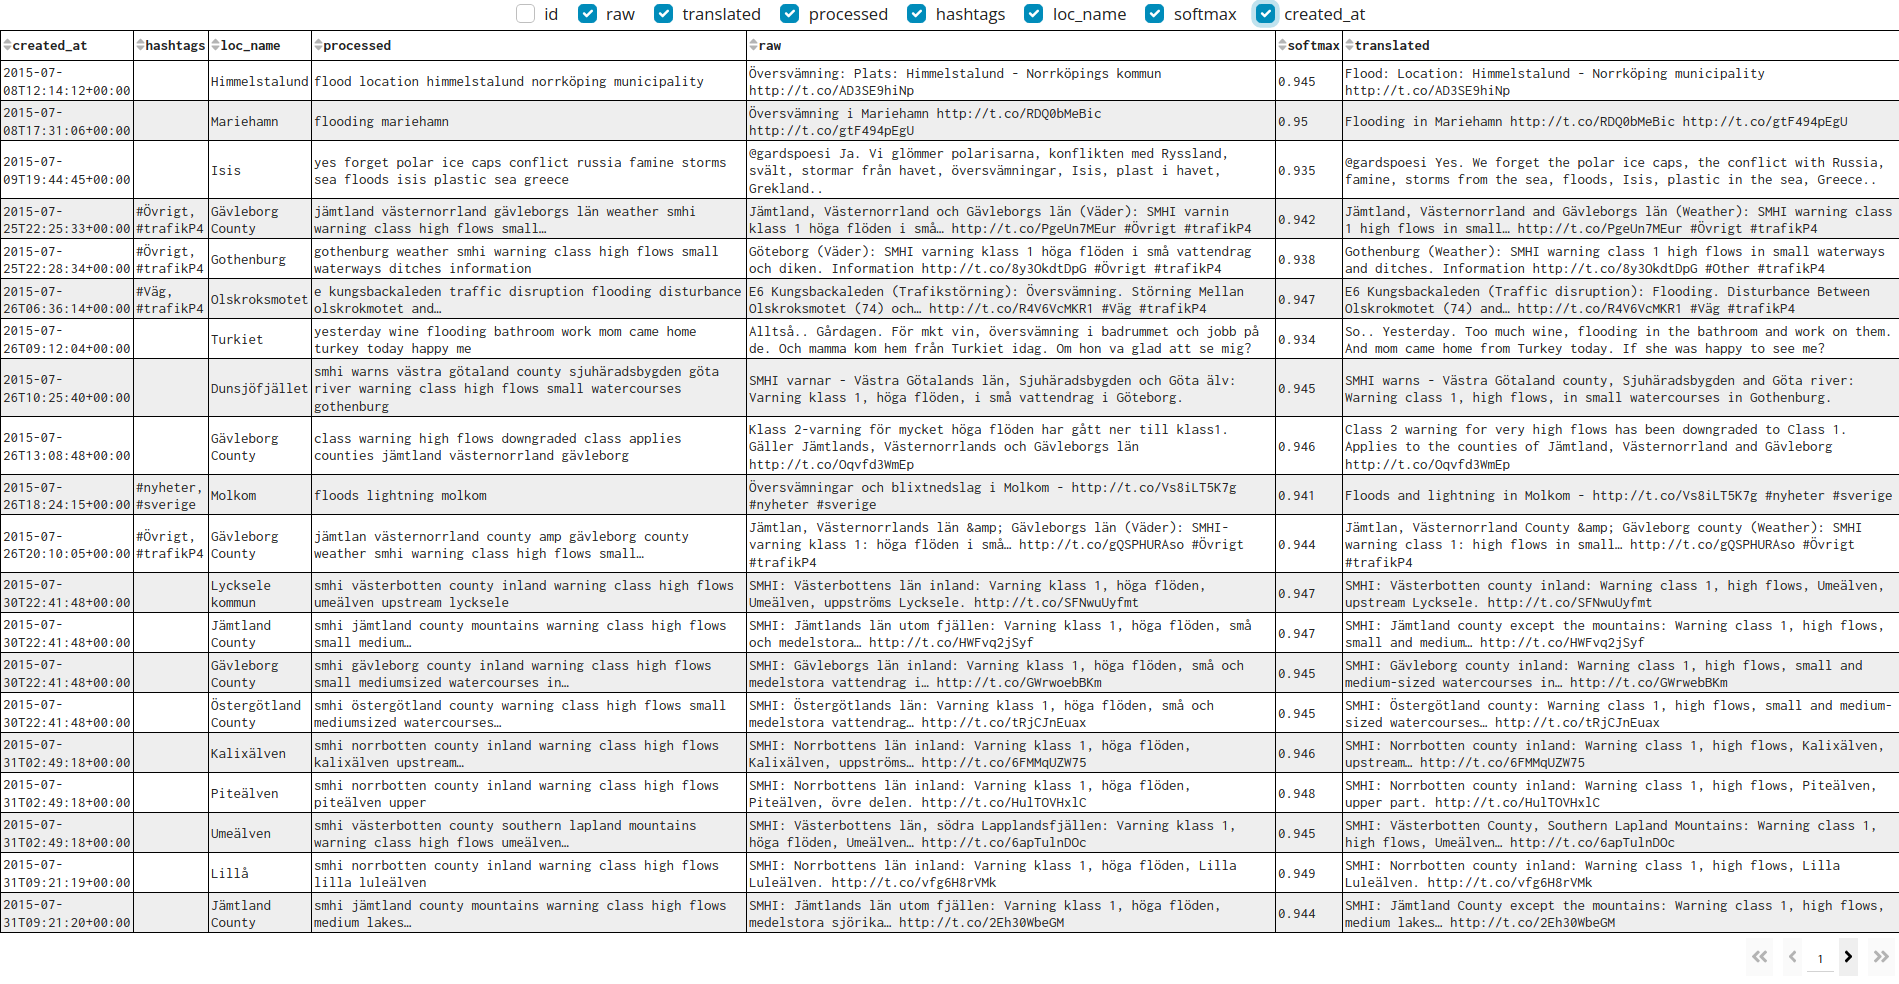
\includegraphics[width=\columnwidth]{./images/tweets_table.png}
\end{center}
\caption{Table showing the tweets}
\label{fig:tweets_table}
\end{figure}

Figure~\ref{fig:scatter} shows a scatter plot for the \ac{t-SNE}'s 2-dimensional space with
\ac{DBSCAN} clustering. The text inputs adjucts the clustering proprties (eps and min samples).
Hovering over the points show a pop-up of the text for the tweets, and the points can be selected
using a box or lasso selection. 

\begin{figure}[H]
\begin{center}
  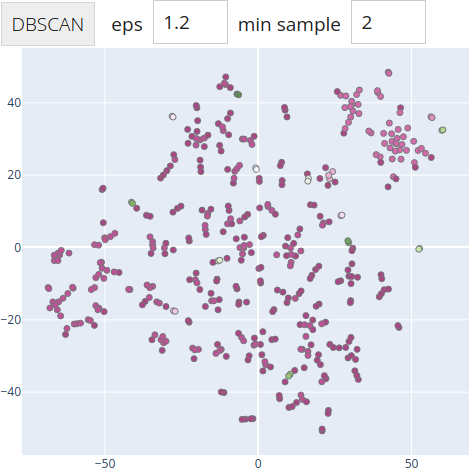
\includegraphics[width=0.666\columnwidth]{./images/scatter.png}
\end{center}
\caption{Scatter plot for \ac{t-SNE}'s space}
\label{fig:scatter}
\end{figure}

The results of \ac{LDA} and \ac{TF-IDF} are displayed in two tables
(shown in Figure~\ref{fig:lda_table} and Figure~\ref{fig:tfidf_table}, respectively)  showing the
frequency of the terms and their mean weights. The number of topics generated by \ac{LDA} can be
changed using a text input, and the tables can be regenerated after changing the selected tweets by
clicking the button. 

\begin{figure}
    \centering
    \begin{subfigure}[b]{0.48\textwidth}
        \centering
        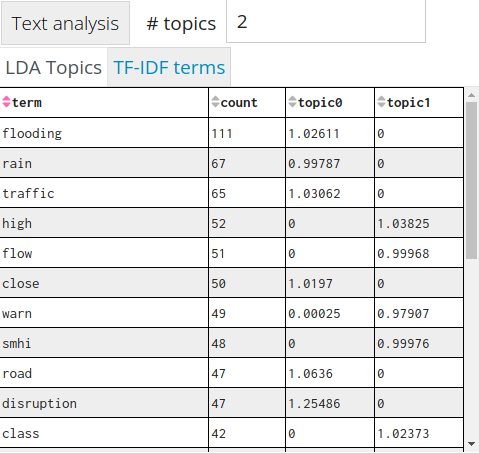
\includegraphics[width=\textwidth]{./images/lda_topics.png}
        \caption{\ac{LDA} topic weights}
        \label{fig:lda_table}
    \end{subfigure}
    \hfill
    \begin{subfigure}[b]{0.48\textwidth}
        \centering
        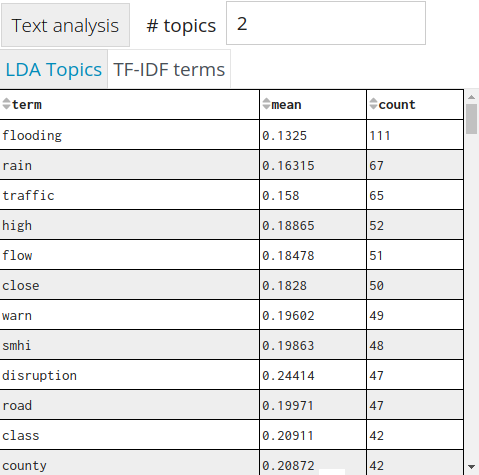
\includegraphics[width=\textwidth, trim={0 0.5cm 0 0},clip]{./images/tf_idf.png}
        \caption{\ac{TF-IDF} weights}
        \label{fig:tfidf_table}
    \end{subfigure}
    \caption{Tables showing terms with respect their frequency and their weights}
    \label{fig:tables_lda_tfidf}
\end{figure}

Lastly, the metadata in Figure~\ref{fig:meta_data} has the following information about the
interface: the total number of tweets, the number of selected tweets, the oldest and newest tweet
creation dates, the total number of locations, the number of selected locations, and a list of
locations' names with the number of their occurrence. Pressing the ``etc.'' button shows a pop-over
with the rest of the locations. 

\begin{figure}[H]
    \begin{center}
        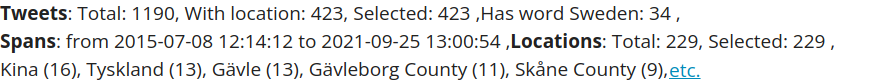
\includegraphics[width=\columnwidth]{./images/meta_data.png}
    \end{center}
    \caption{Metadata about the visual interface}
    \label{fig:meta_data}
\end{figure}
